\documentclass[MasterThesisMain.tex]{subfiles}
\begin{document}
\chapter{Analysis} \label{ch:analysis}

\section{Light source fluctuation}
Looking at equation \ref{eq:nanocalcreflect}, which is the expression for how the spectrometer measures the reflectance of light from the thin films reveils the importance of the intensity of light being used in the measurement. A fluctuation in the intensity of light gives repercussions for the reference measurement and dark measurement taken as both measurements are not correct at the point they were taken and will not correct in future measurements. The question is how long does a reference and dark measurement remain valid. This study aims is to shed light on this problem. The scripts used can be found in appendix \ref{app:Lightstudy}. The thin film used is polystyrene and a total of $14$ measurements were done in the SVA experimental chamber. A measurement was taken every $\SI{30}{\minute}$, a measurement was made manually at $10$:$47$ and the automatic measurements commenced at $11$:$19$. The measurements can be seen plotted together in figure \ref{fig:daytotal}. Distinguishing which curve belongs to which time is not possible because of the limited amount of plotting colours, but two groups of reflectance curves can be seen at the $\SI{600}{\nano\meter}$ mark and again at the $\SI{900}{\nano\meter}$ mark.
  
\begin{figure}
\centering
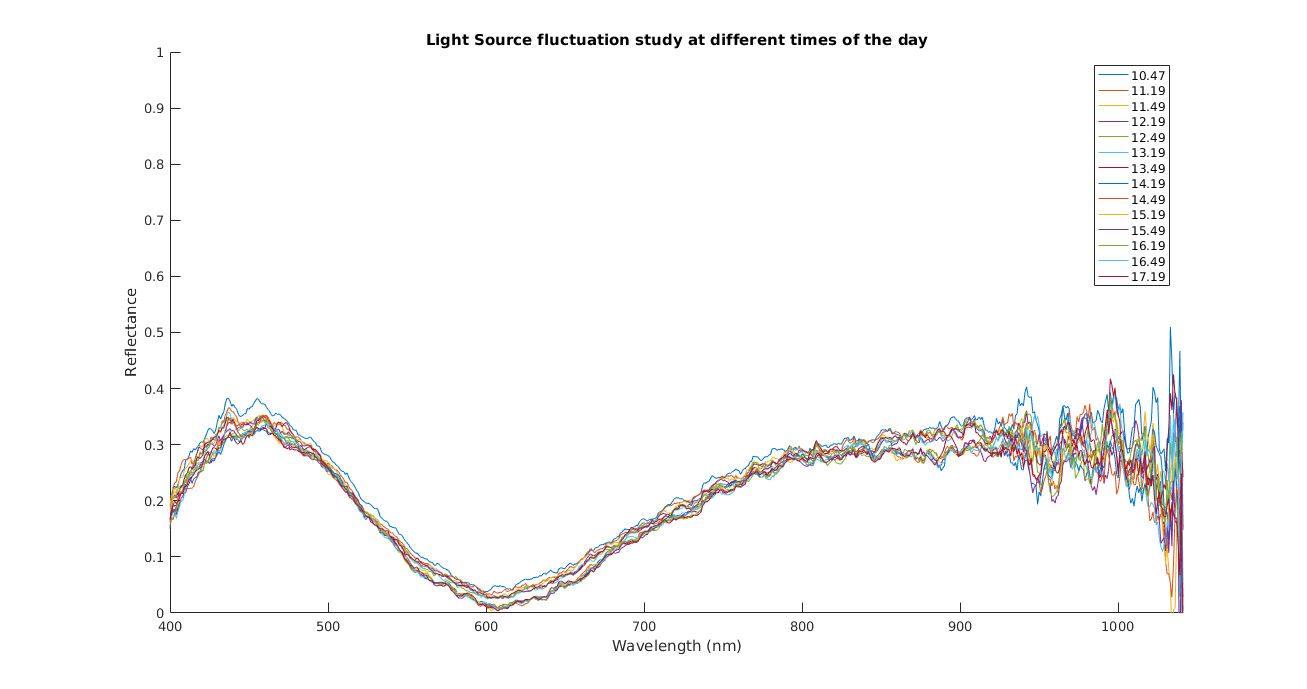
\includegraphics[width=\textwidth]{fluctstudytotal.png}
\caption{14 reflectance measurements plotted representing a reflectance measurement taken every $30$ minutes. Distinguishing which curves belongs to which time is not possible, but two groups of reflectance curves can be seen at the $\SI{600}{\nano\meter}$ mark and again at the $\SI{900}{\nano\meter}$ mark.}
\label{fig:daytotal}
\end{figure}

Figures \ref{fig:day1} and \ref{fig:day2} show the first reflectance measurement taken at $10:47$ plotted against the reflectance measurements taken at the times $12$:$19$, $13$:$49$, and $15$:$19$, $17$:$19$ respectively. In figure \ref{fig:day1}, the reflectance measurements lie close to one another. In figure \ref{fig:day2}, the drop in reflectance seen at the $\SI{600}{\nano\meter}$ mark starts at the time $15$:$19$ and continues onwards. 

\begin{figure}
\centering
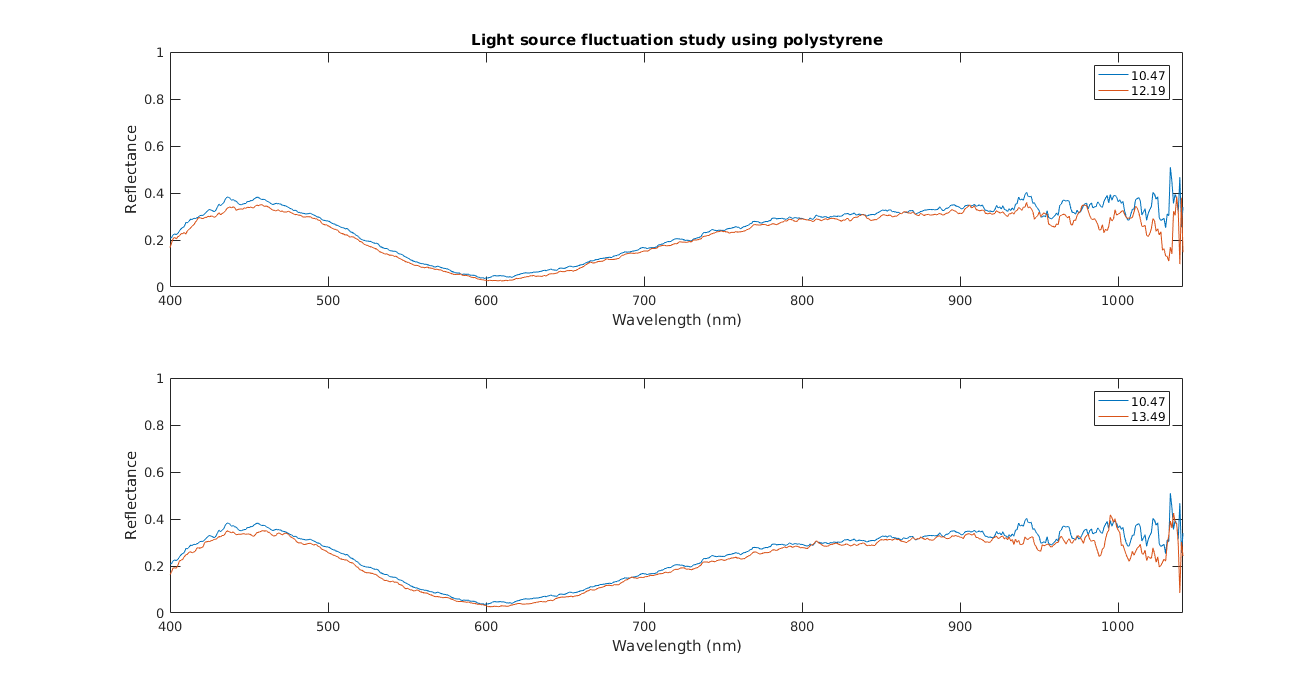
\includegraphics[width=\textwidth]{lightfluct1.png}
\caption{The reflectance measurement taken at $10$:$47$ plotted with both $12$:$19$ and $13$:$49$. It can be seen that there is a small deviation but lay close to one another.}
\label{fig:day1}
\end{figure}

\begin{figure}
\centering
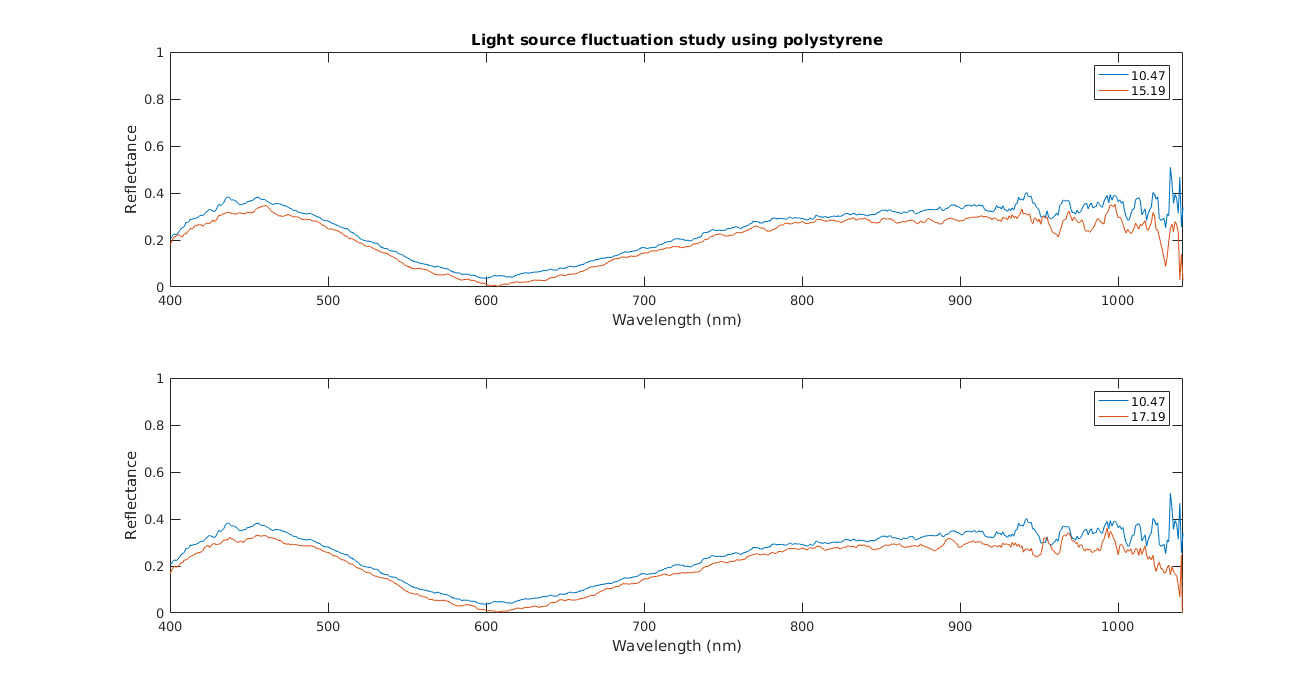
\includegraphics[width=\textwidth]{lightfluct2.png}
\caption{The reflectance measurement taken at $10$:$47$ plotted with both $15$:$19$ and $17$:$49$. It can be seen that the deviation between the reflectance data is increasing.}
\label{fig:day2}
\end{figure}

The reflectance difference has been plotted in figure \ref{fig:day3}. It can be seen that the difference of $10$:$47$ plotted with both $12$:$19$ and $13$:$49$ lie on top of one another and the difference of $10$:$47$ plotted with both $15$:$19$ and $17$:$49$ lie on top of one another. There is a clear difference between the two groups of plots.

\begin{figure}
\centering
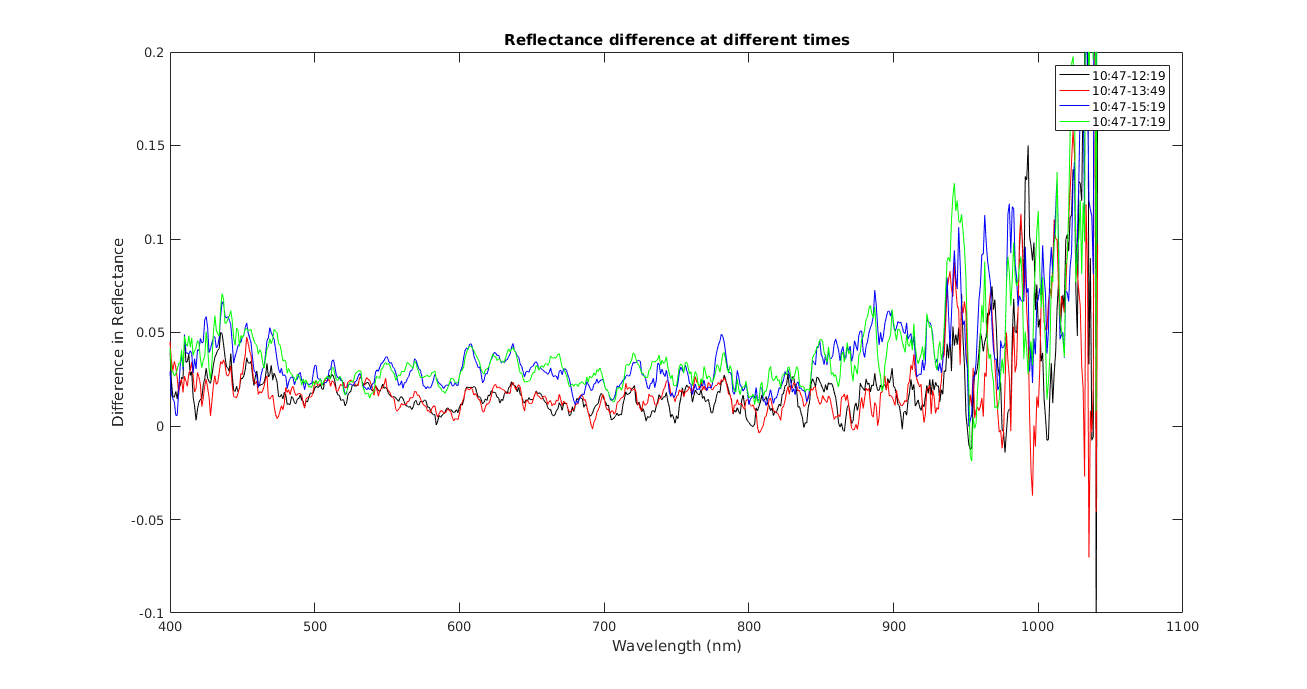
\includegraphics[width=\textwidth]{refldiffday.png}
\caption{The reflectance difference between the reflectance data at $10$:$47$ and the other times $12$:$19$, $13$:$49$, $15$:$19$ and $17$:$19$ are shown. It can be seen that the reflectance data groups itself into two, first group with times $12$:$19$ and $13$:$49$ and the second group $15$:$19$, $17$:$19$.}
\label{fig:day3}
\end{figure}
\pagebreak
The conclusion to this study is that there is a $3$ hour window where the variation in the intensity from the light source does not impact the reflectance measurements. Beyond the $3$ hour period, the reflectance difference increases and can impact the reflectance measurements.

	
\section{Nano-Calc Simulated Reflectance Curves}
The Nano-Calc software does not go into detail how it models and analyses the reflectance curves, a little study was need to understand the process better and test if the software uses Fresnel equation and if the functions written by myself could reproduce these curves. Using the Nano-Calc software, simulated reflectance curves were produced from three models. The first model consists of of ambient of air refractive index $1$, and the silicon substrate, the Fresnel equation can be seen in equation \ref{eq:a-srefl}. The reflectance curves can be seen in figure \ref{fig:simmodelsubst}. The second model consists of ambient of air refractive index $1$, a thin film of polymer with homogeneous refractive index $1.5$ and thickness $\SI{1000}{\nano\meter}$ and the silicon substrate, the fresnel equation can be seen in equation \ref{eq:2layerreflect}. The reflectance curves can be seen in figure \ref{fig:simmodel1}. The third model consists of ambient of air refractive index $1$, a thin film of polymer using the Cauchy dispersion equation $A=1.4450$, $B=3 \cdot 10^4$ and $C=4 \cdot 10^7$, a silicon oxide layer with thickness $\SI{2}{\nano\meter}$ and the silicon substrate, the fresnel equation can be seen in equation \ref{eq:multilayer} . The reflectance curves can be seen in figure \ref{fig:simmodel2}. The Cauchy dispersion equation is an empirical equation describing how the refractive index varies with respect to wavelength. The Cauchy dispersion equation is defined as:

\begin{equation}
n(\lambda) = A + \frac{B}{\lambda^2} + \frac{C}{\lambda^4},
\end{equation}
where $\lambda$ is the wavelength. This is the only time the Cauchy dispersion equation will be used. The coefficient A describes the refractive index when the terms with wavelength become less dominant. The Cauchy dispersion equation has not been implemented into the fitting protocol used on the reflectance data of the homopolymers and block copolymer. It is interesting nonetheless to look at the refractive index of the polymers as a function of wavelength. The cauchy dispersion equation has been plotted in figure \ref{fig:dispshort}. The coefficient have been found experimentally using ellipsometry. It can be seen in figure \ref{fig:dispshort} that polystyrene is the only polymer which is close to a constant refractive index. Polyisoprene and polystyrene-b-polyisoprenes refractive index diverges alot compared to the constant refractive index. Since the fitting of the homopolymers and Block copolymer reflectance data is done across the interval $[450,900]$, i have included the amount in which the refractive index deviates from the constant refractive index at $\SI{450}{\nano\meter}$ in red font.   

\begin{figure}[H]
\centering
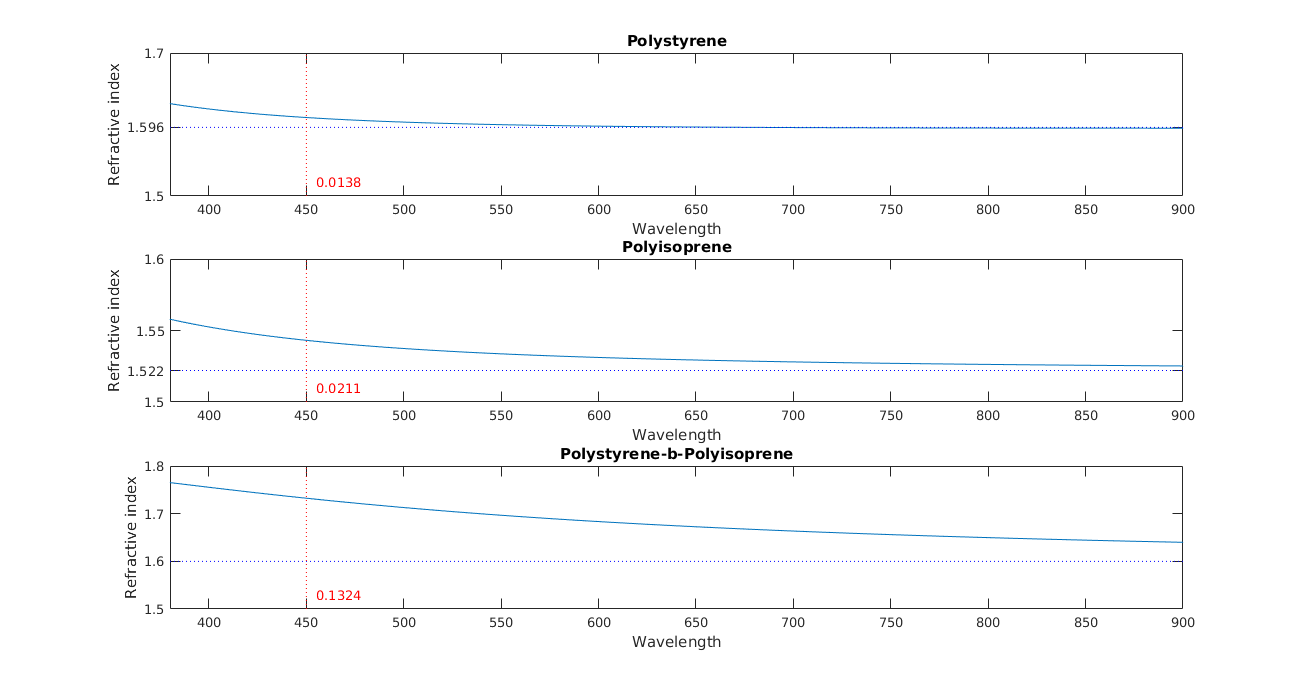
\includegraphics[width = \textwidth]{dispersionshort.png}
\caption{The cauchy dispersion equation has been plotted for Polystyrene, Polyisoprene and Polystyrene-b-Polyisoprene. The amount in which the refractive index deviates from the constant refractive index at $\SI{450}{\nano\meter}$ has been included in red font.}
\label{fig:dispshort}
\end{figure} 

When modelling the Fresnel equations, both the refractive index and absorption index for the silicon oxide layer and silicon substrate have been used for the complex refractive index. The dispersion for both the silicon oxide layer and silicon substrate have been taken from the Nano-Calc software and the graphs and script to produce the graphs can be seen in appendix \ref{app:dispersion}.  

\begin{figure}[H]
\centering
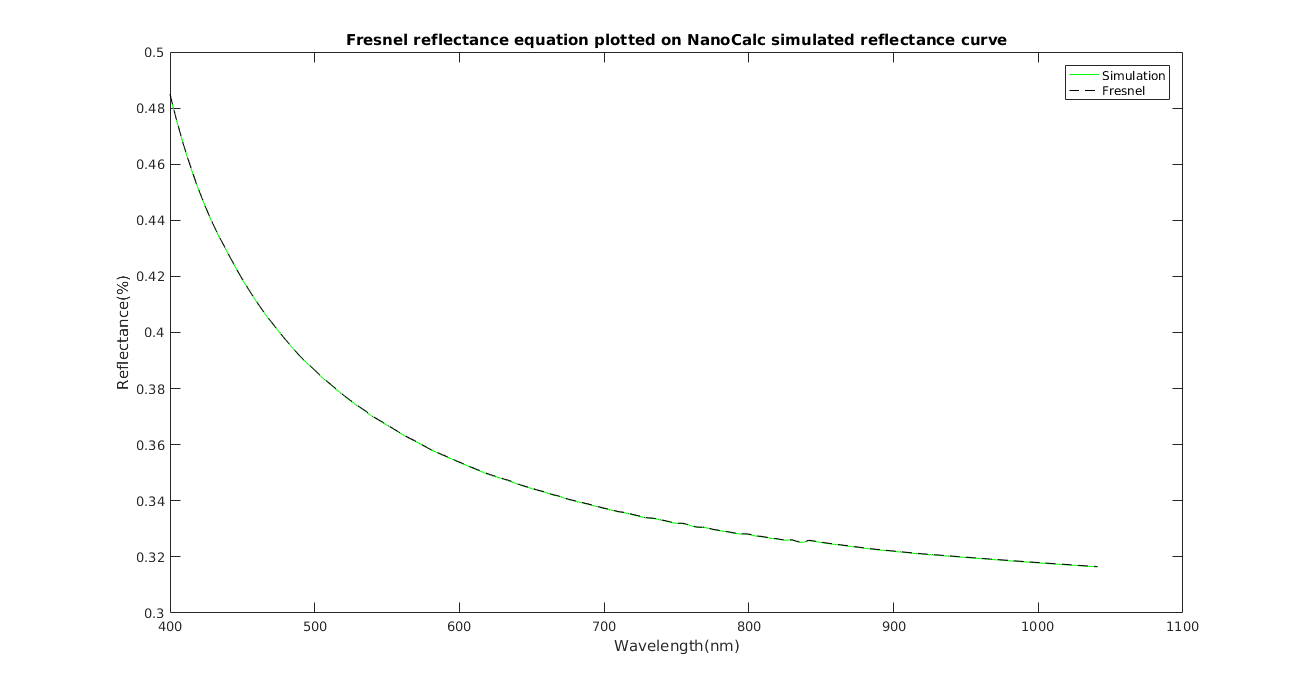
\includegraphics[width=\textwidth]{simcurvesubst.png}
\caption{Simulated curve of the model plotted with the green curve, consists of ambient of air refractive index $1$, and the silicon substrate. The Fresnel equations plotted with the black dashed curve consists of the same model. It can be seen that the two curves fall upon each other.}
\label{fig:simmodelsubst}
\end{figure}

\begin{figure}[H]
\centering
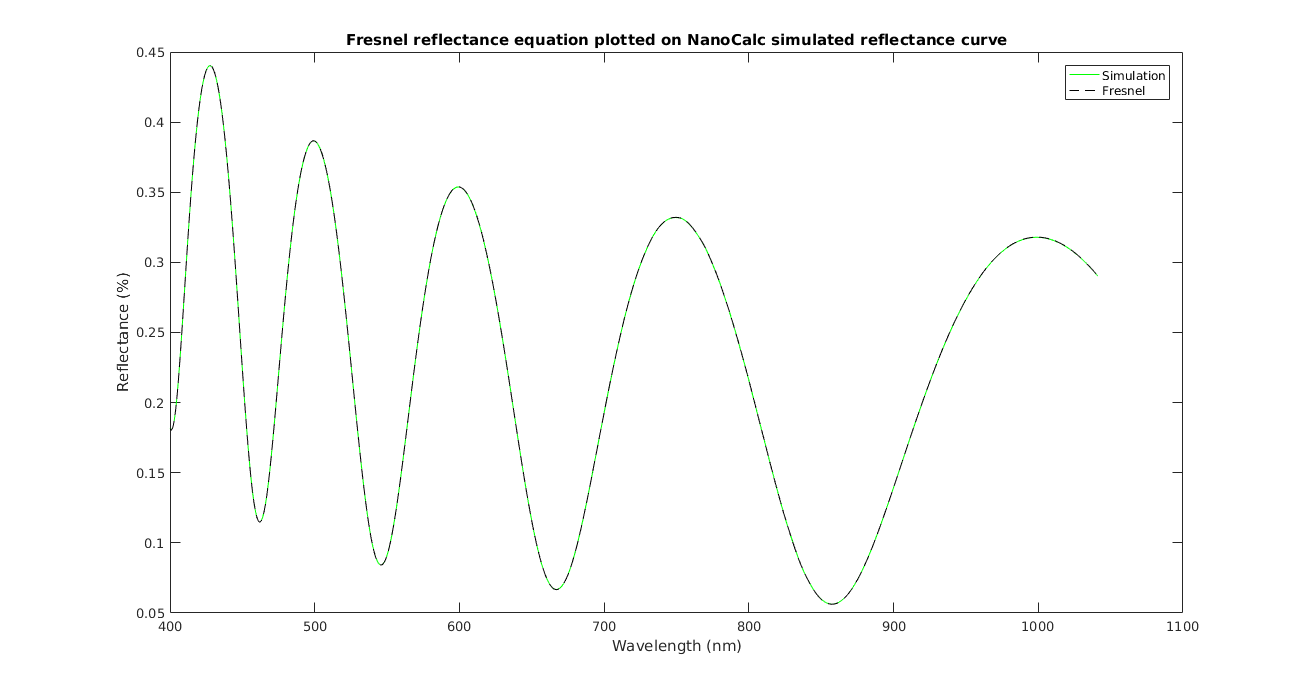
\includegraphics[width=\textwidth]{simcurve.png}
\caption{Simulated curve of the model plotted with the green curve, consists of ambient of air refractive index $1$, a thin film of polymer with homogeneous refractive index $1.5$ and thickness $\SI{1000}{\nano\meter}$ and the silicon substrate. The Fresnel equations plotted with the black dashed curve consists of the same model. It can be seen that the two curves fall upon each other.}
\label{fig:simmodel1}
\end{figure}

\begin{figure}[H]
\centering
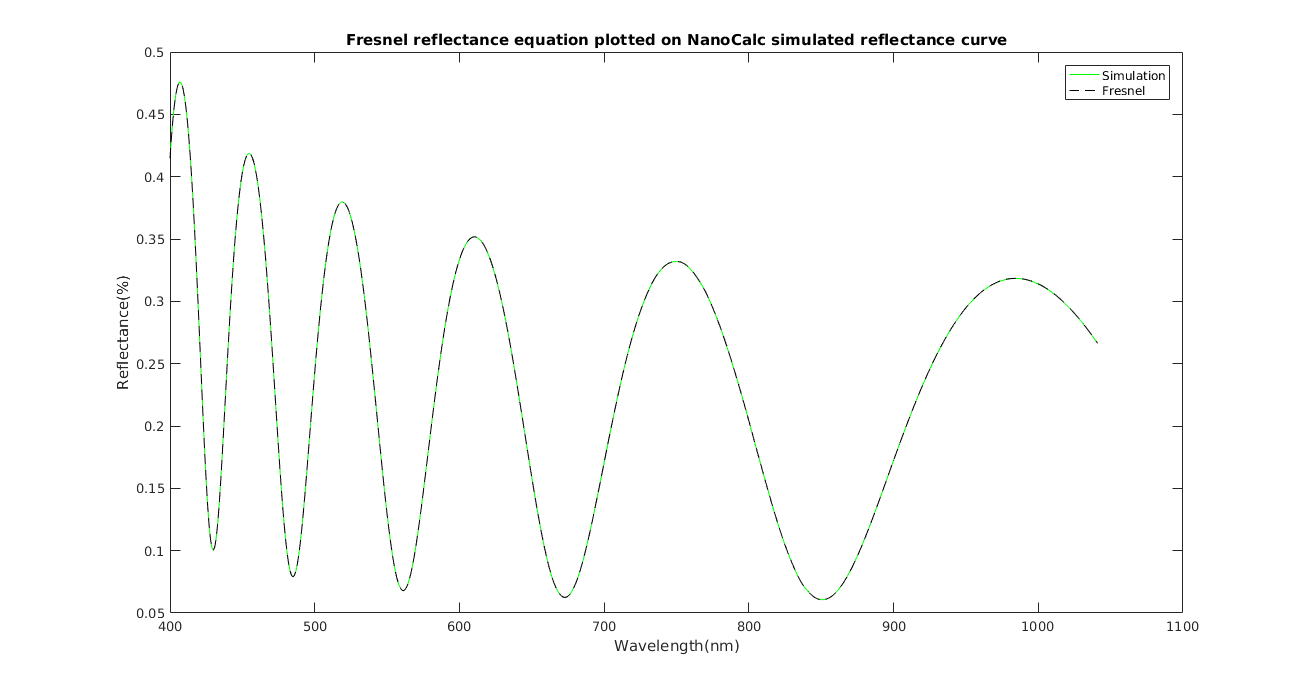
\includegraphics[width=\textwidth]{simcurvesiox.png}
\caption{Simulated curve of the model plotted with the green curve, consists of ambient of air refractive index $1$, a thin film of polymer using the Cauchy dispersion equation $A=1.4450$, $B=3 \cdot 10^4$ and $C=4 \cdot 10^7$, a silicon oxide layer with thickness $\SI{2}{\nano\meter}$ and the silicon substrate. The Fresnel equations plotted with the black dashed curve consists of the same model. It can be seen that the two curves fall upon each other.}
\label{fig:simmodel2}
\end{figure}

Two conclusions have been drawn from this study. The first is that the Fresnel equations implemented by myself in the script used in this chapter can reproduce the simulated curves used by the Nano-Calc software to model the reflectance curves. The second is that the fitting protocol for the reflectance curves will not implement the Cauchy dispersion for refractive index because it is not fully understood and it is not something the optical spectral reflectance method can fully reveil.    
	
\section{Solvent vapour annealing ambient study}
During solvent vapour annealing, nitrogen flow through the bubbler increases, increasing the toluene vapour present in the chamber. The question arises, does the refractive index of the ambient increase with the increase of toluene vapour available in the chamber. A blank silicon wafer has been used for this study. Upon the silicon wafer lies a silicon oxide layer modelled to have a thickness of $\SI{2}{\nano\meter}$. The refractive index has been allowed to vary between $1$ through to $2$ with a step of $0.1$. The fitting protocol loops through each refractive index, calculating the theoretical reflectance curve from the fresnel equation \ref{eq:a-srefl}. The mean square error has been calculated for each loop and the minimum has been found and the refractive index saved into a file. The swelling protocol used has been outlined in section \ref{sec:svaprotocol} and can be seen in figure \ref{fig:slowslow}. From the mean square error fitting, the refractive index varied between $1$ through to $1.3$ through the course of swelling, this can be seen in figure \ref{fig:ambientrefr}. The dotted vertical line represent the different stages in the solvent vapour annealing and the maximum flow through the bubbler has been highlighted with the red vertical dots.

\begin{figure}
\centering
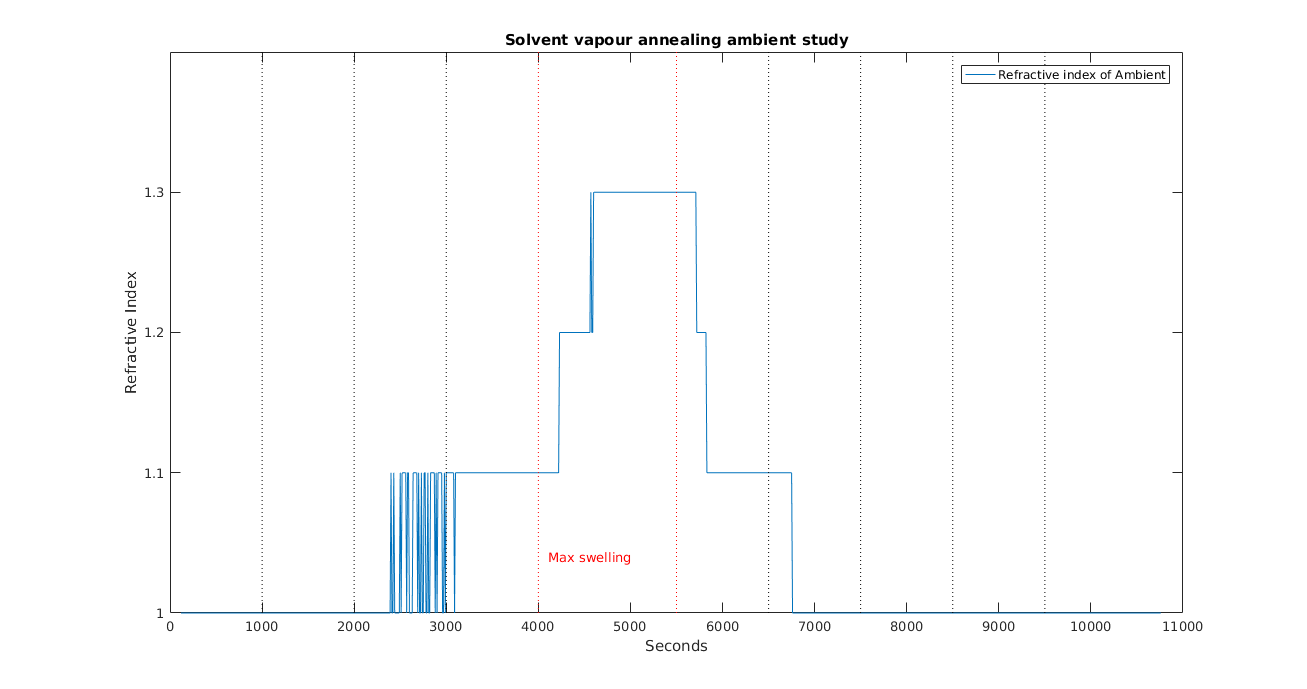
\includegraphics[width=\textwidth]{ambientstudyrefr.png}
\caption{The refractive index of the ambient has been plotted. The refractive index has been fitted by plotting the theoretical reflectance curve from the fresnel equation \ref{eq:a-srefl} and calculating the mean square error. The refractive index from the lowest mean square error has been used per reflectance measurement. The dotted vertical lines represent the swelling and deswelling step outlines in section \ref{sec:svaprotocol}. The red dotted lines indicate the period where there is maximum flow through the bubbler.}
\label{fig:ambientrefr}
\end{figure}

The mean square error for each reflectance measurement is shown in figure \ref{fig:ambientmse}. It can be seen between the $2000$ and $3000$ second mark the refractive index is erratic, this is mirrored in the increase in the mean square error. The same happens when the fitting increases the refractive index to $1.3$, the mean square error increase then falls. During the deswelling period there is an increase in mean square error when every the refractive index decreases. When watching the reflectance data play like a movie, it can be seen that the reflectance does decrease. The decrease in reflectance data in shown in figure \ref{fig:ambientreflectance}. As stated the wafer used is a silicon wafer with an oxide layer. Both layer are unable to take up vapour and their thickness cannot increase, thus the variable in this set up is the ambient refractive index.

\begin{figure}
\centering
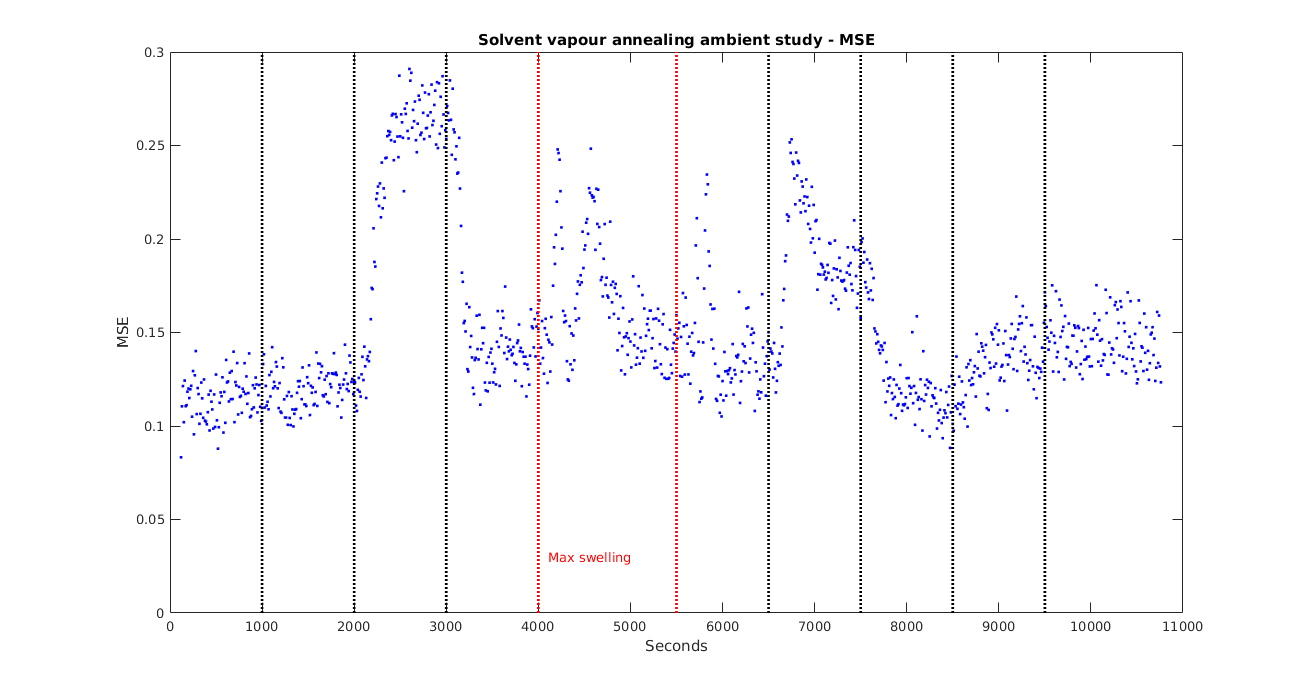
\includegraphics[width = \textwidth]{ambientstudymse.png}
\caption{The mean square error has been plotted as a function of time. The frames have been captured every $10$ time. It can be seen that the error increase every time the modelling increases or decreases the refractive index but stabilises back to a level close error before the change in refractive index.}
\label{fig:ambientmse}
\end{figure}

\begin{figure}
\centering
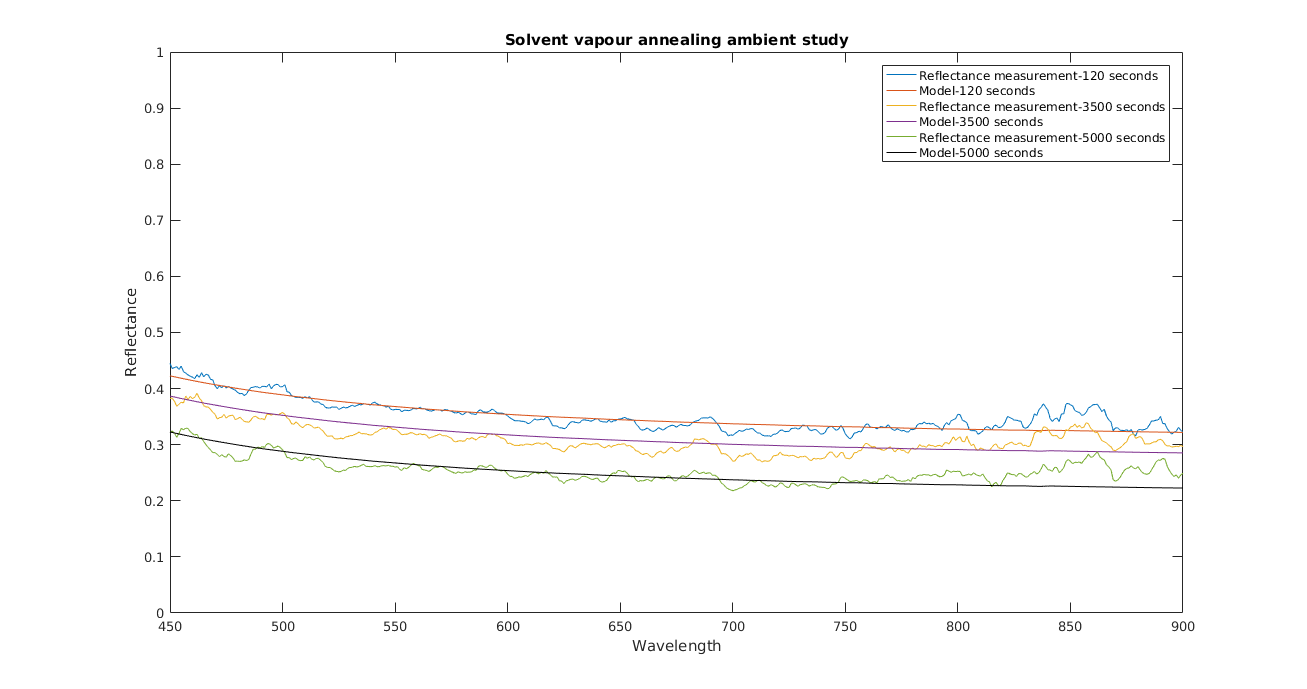
\includegraphics[width = \textwidth]{ambientreflectancestep.png}
\caption{Three reflectance curves has been plotted to show how the reflectance decreases during solvent vapour annealing when the toluene vapour in the chamber increases. The fresnel reflectance model equation \ref{eq:a-srefl} has been plotted for each stage in the solvent vapour annealing. The measurement at time $120$ second is modelled with a refractive index of $1$. The measurement at time $3500$ time is modelled with a refractive index of $1.1$. The third measurement at time $5000$ time is modelled with a refractive index of $1.3$.}
\label{fig:ambientreflectance}
\end{figure}

The conclusion to this study is that the ambient in the solvent vapour annealing chamber increase during the swelling. The interval in which the refractive index of the ambient increase, lies between $1$ and $1.3$. 
	
\section{Polystyrene}
Polystyrene with a static measured thickness of $\SI{275.5}{\nano\meter}$ and a refractive index $1.5975$, has been placed into the solvent vapour annealing chamber and swelled using the swelling protocol outlines in section \ref{sec:svaprotocol}. The ambient refractive index has been bounded to the interval $[1,1.3]$ with a step size $0.1$. The thin film refractive index has been bounded to the interval $[1.1,2]$ with a step size $0.1$. The thin film thickness bounded to the interval $[\SI{250}{\nano\meter},\SI{600}{\nano\meter}]$ with step size $1$ and the silicon oxide thickness set to $\SI{2}{\nano\meter}$. Figure \ref{fig:PSswelling1} shows the values found using the fitting protocol using the mean square error and have been as a function of time.  Vertical dotted lines has been added to represent at what point the the swelling protocol has increased and decreased the nitrogen and toluene vapour. Horizontal lines has been added to the thickness plot to help the reader. The thickness of the polystyrene shows a slow uptake of the toluene vapour during the first $4000$ seconds during this time the refractive index for the polystyrene has increased by $0.4$ to a refractive index of $2$. The refractive index jump from $1.6$ to $1.7$ passed the $1000$ seconds mark and the jump from $1.8$ to $2$ around the $3000$ second mark coincide with jumps in the refractive index of the ambient. The refractive index of the ambient increases slowly over the course of the first $4000$ seconds, increase after the nitrogen through the toluene has increased. There are areas in the figures where there is noise, jumps back and forth from values and a sudden decrease in thickness. The fitting has trouble fitting around the $\SI{450}{\nano\meter}$ and $\SI{500}{\nano\meter}$ interval, i believe this is the cause of the noise. This is also reflected in the mean square error figure \ref{fig:PSswelling2}. The increase of the mean square error at $1500$ mark coincide with the noise in the refractive index of the ambient and thin film, and thickness, figure \ref{fig:PSswelling1}. The increase of the square error at $2500$ and $3000$ mark shows sudden drops in the thickness values which also coincide with increase of the refractive index of the thin film. During the maximum swelling interval the mean square error increases from $0.1$ to $1$. The reflectance during this time decreases creating a gap between the fresnel reflectance equations and reflectance measurement increasing the mean square error. When a slow drying commences at the $5500$ second mark, the thickness and mean square error values drops significantly. The swelling from $\SI{300}{\nano\meter}$ to $\SI{450}{\nano\meter}$ takes roughly $1500$ seconds and deswelling to roughly the same thickness takes $500$ seconds is very interesting. The increase in the mean square error after the $6500$ second mark can be because of the noise in the thin film refractive index. The solvent concentration in the thin film as a function of time is shown in figure \ref{fig:PSswelling3}.        

\begin{figure}
\centering
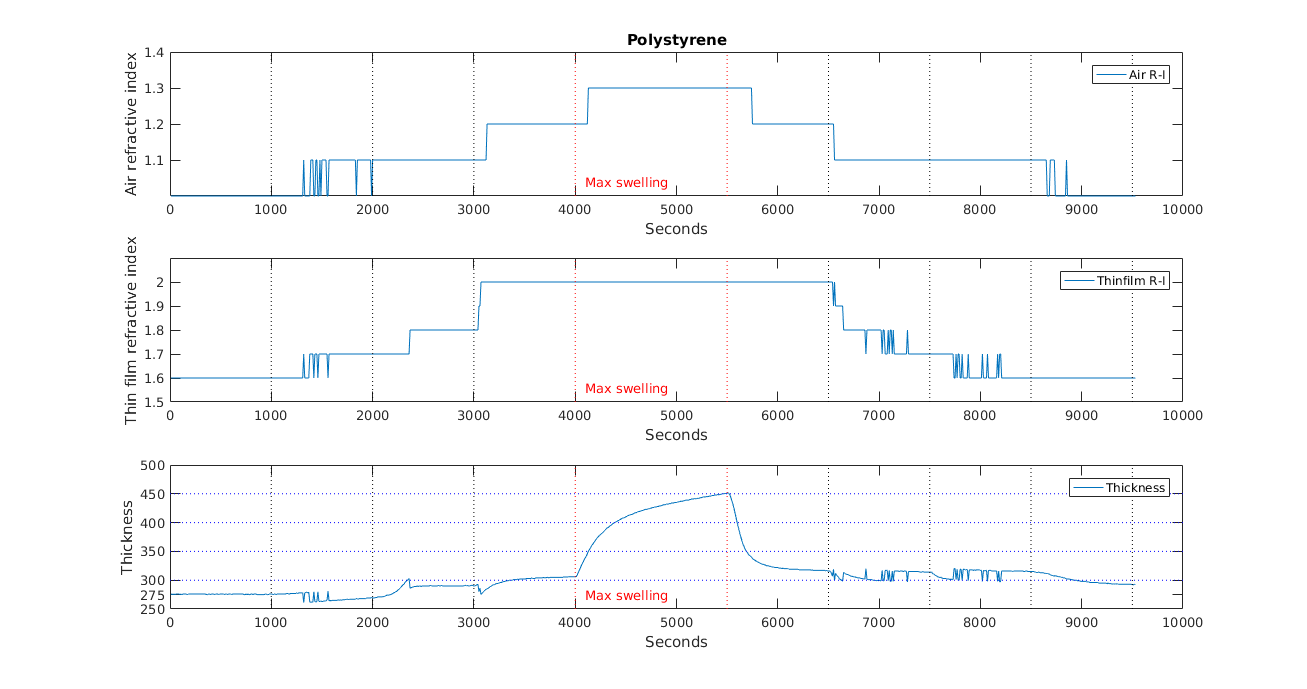
\includegraphics[width = \textwidth]{PSswelling1.png}
\caption{The values for the refractive index for the ambient and thin film, and the thickness has been plotted as a function of time for polystyrene. The values have been found using the fitting protocol outlined in \ref{sec:fitting}. Vertical dotted lines have been added to denote when there is increases and decreases of nitrogen and nitrogen through the toluene. The area between the red vertical dotted lines denote the maximum flow through the toluene.}
\label{fig:PSswelling1}
\end{figure}


\begin{figure}
\centering
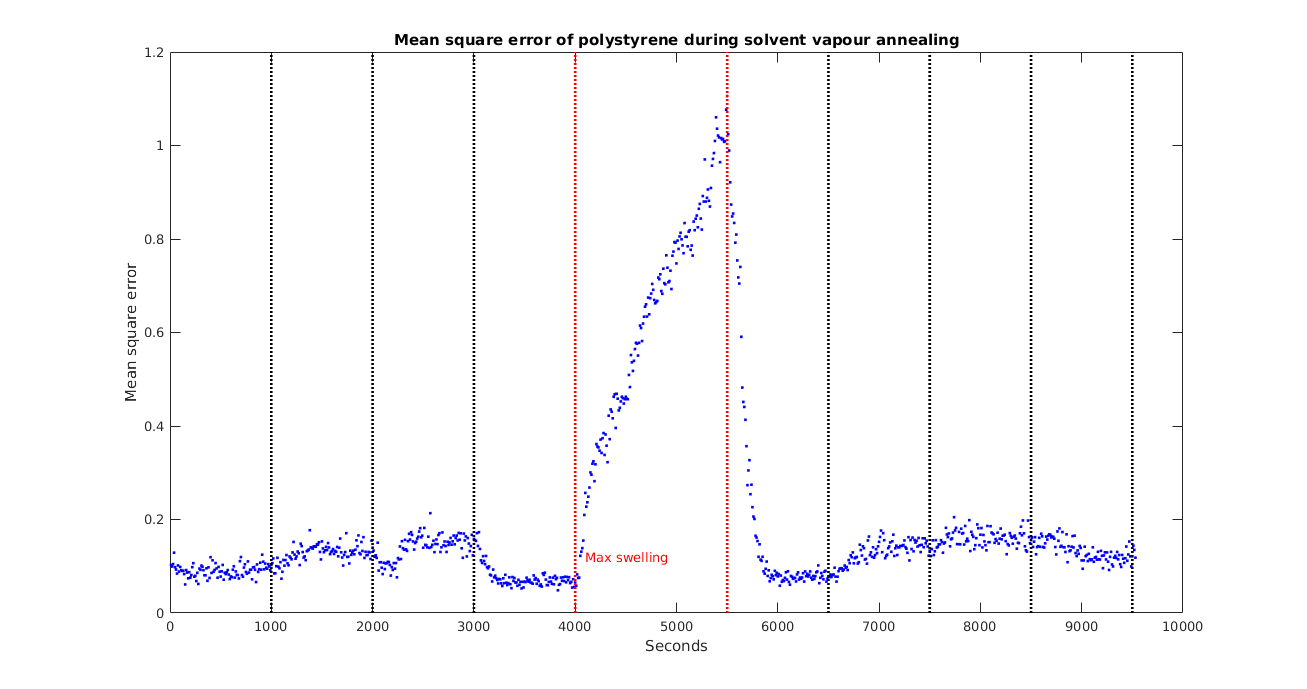
\includegraphics[width = \textwidth]{PSswelling2.png}
\caption{The mean square error has been plotted as a function of time. The mean square error can be seen to increase at the $1500$ and $2500$ mark due to noise in the modelling and drop in thickness values. The mean square error increases from $0.1$ to $1$ during the max toluene swelling, this is due to the reflectance decreasing during this time and creating a gap between the fresnel reflectance equation and reflectance. The increase in the mean square error after the $6500$ second mark can be because of the noise in the thin film refractive index.}
\label{fig:PSswelling2}
\end{figure}

\begin{figure}
\centering
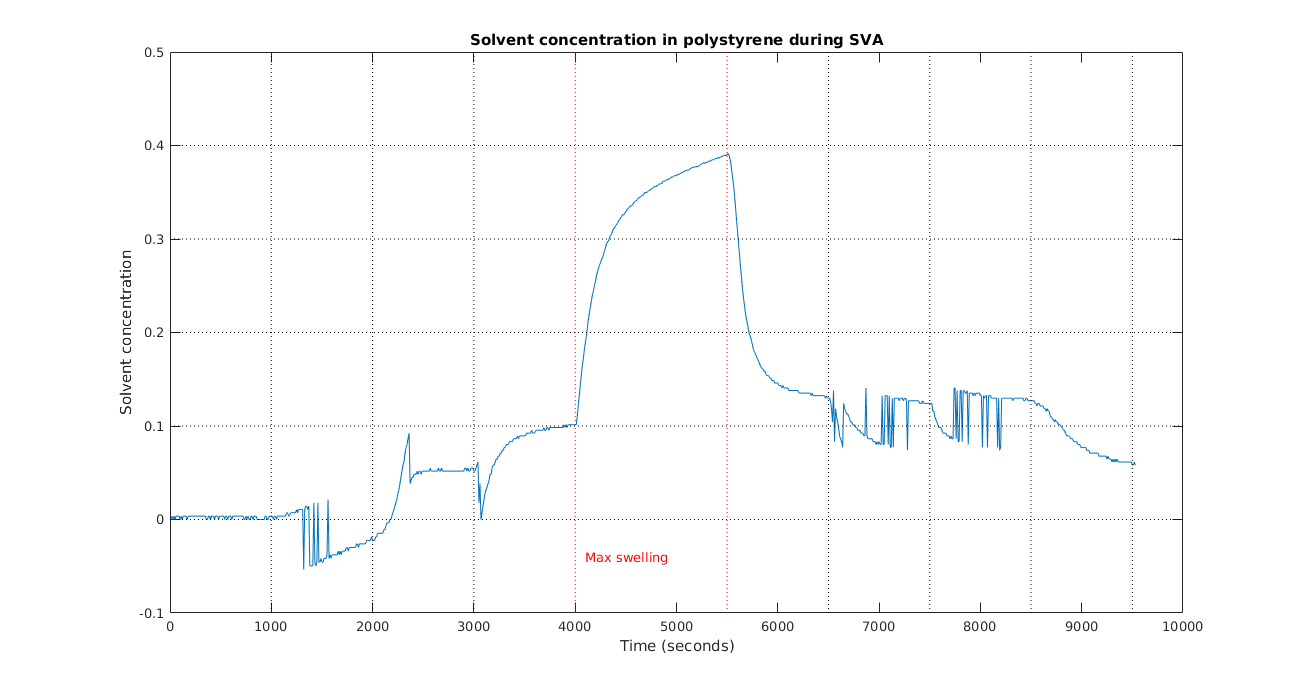
\includegraphics[width = \textwidth]{PSswelling3.png}
\caption{The solvent concentration in the polystyrene as a function of time.}
\label{fig:PSswelling3}
\end{figure}
	
\section{Polyisoprene}
Polyisoprene has been solvent vapour annealed using the protocol outlines in section \ref{sec:svaprotocol}

\begin{figure}[H]
\centering
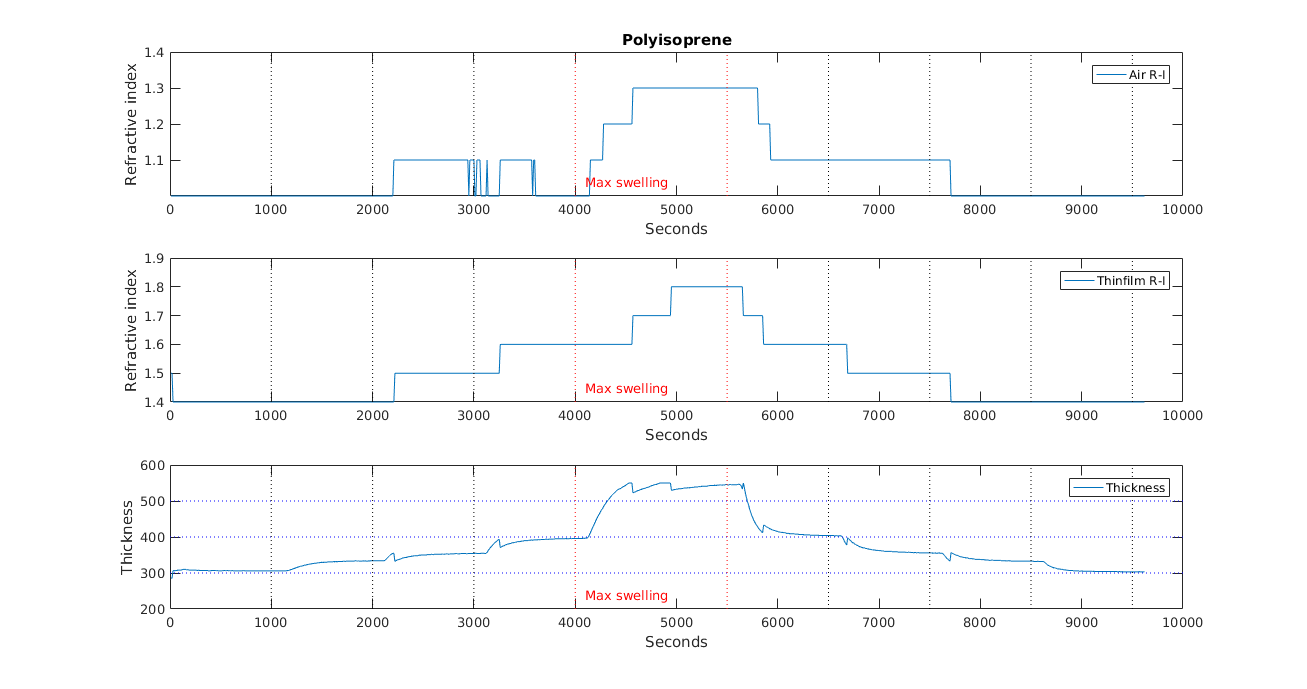
\includegraphics[width = \textwidth]{PIswelling1.png}
\caption{}
\label{fig:PIswelling1}
\end{figure}

\begin{figure}[H]
\centering
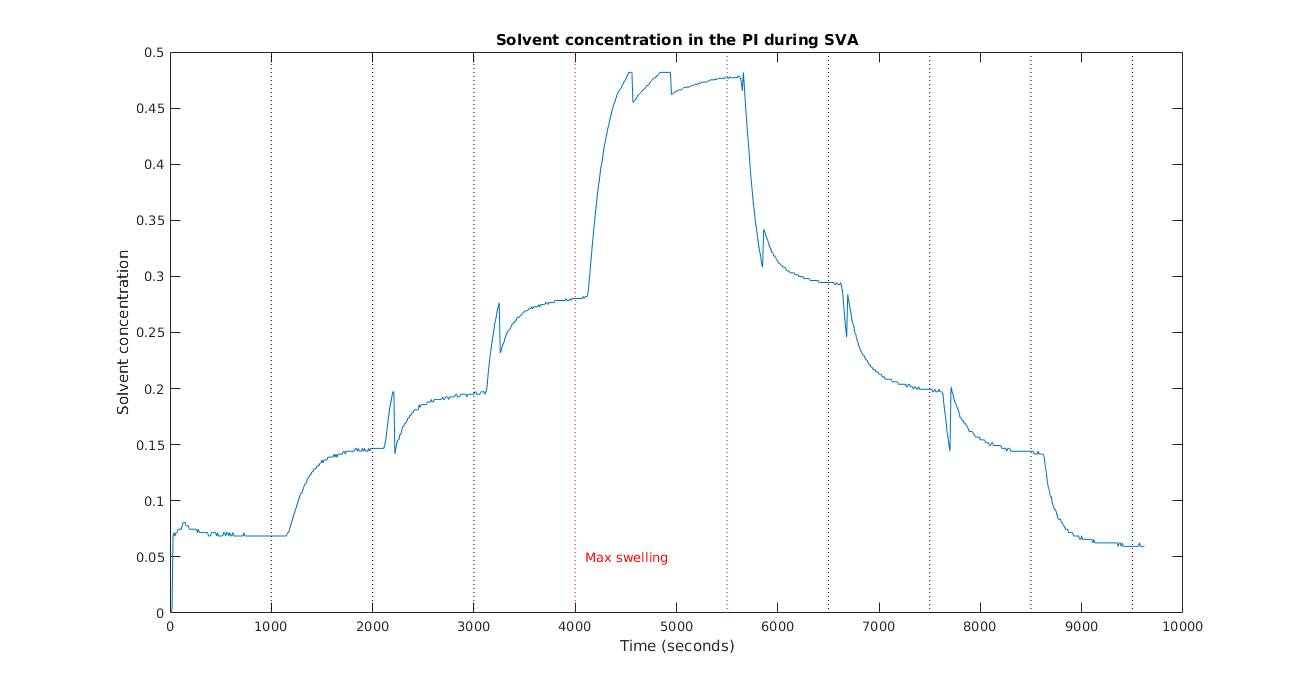
\includegraphics[width = \textwidth]{PIswelling2.png}
\caption{}
\label{fig:PIswelling2}
\end{figure}

\begin{figure}[H]
\centering
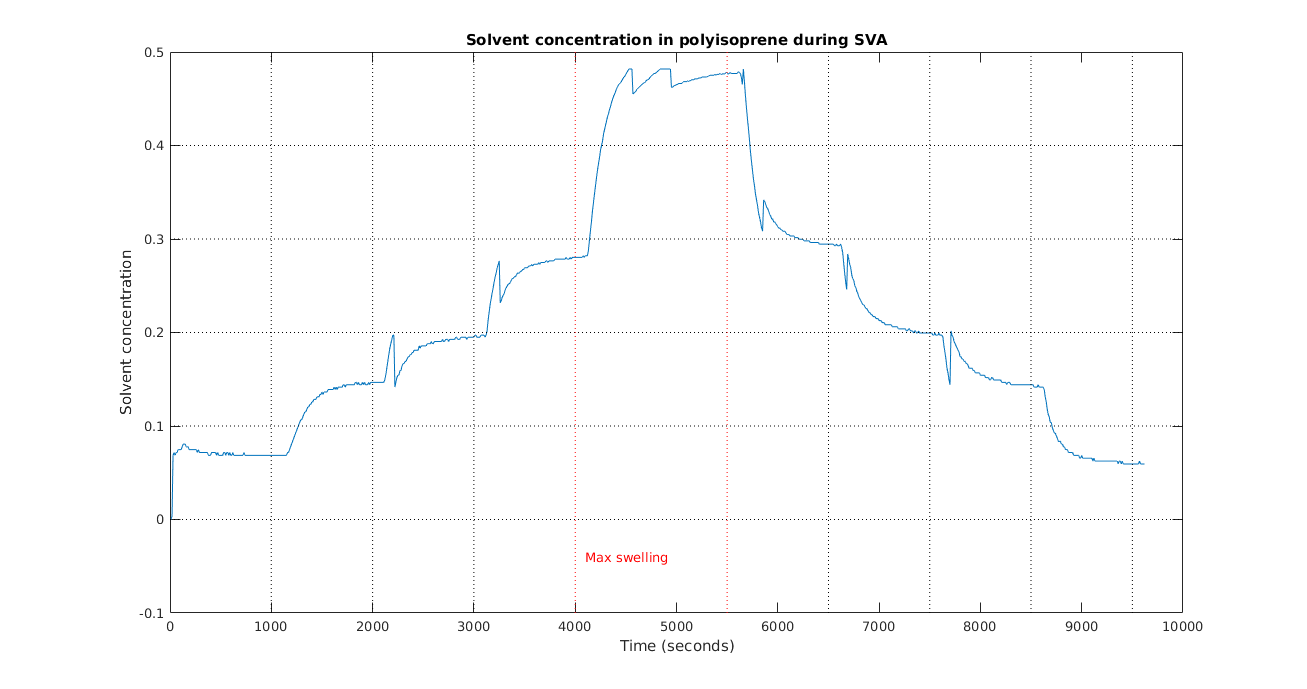
\includegraphics[width = \textwidth]{PIswelling3.png}
\caption{}
\label{fig:PIswelling3}
\end{figure}
	
\section{Polystyrene-b-polyisoprene}


\end{document}